\documentclass[10pt, brown]{beamer}
\usetheme{Warsaw}
\usepackage[MeX]{polski}
\usepackage[cp1250]{inputenc}  % Polskie literki...
\usepackage[polish]{babel}     %
\usepackage{parskip}
\usepackage{latexsym,gensymb,amsmath,amssymb,amsthm}
\usepackage{graphicx}
%\usepackage{verbatim}
\usepackage{ragged2e}
\usepackage{url}
%\setlength{\parindent}{0pt}
%\setlength{\parskip}{1ex}
\renewcommand{\qedsymbol}{$\square$}
\newenvironment{dowod}{{\bf Dow�d.}}{\hfill\rule[0.025cm]{0.21cm}{0.21cm}}
\newtheorem{tw}{Twierdzenie}
\newtheorem{fakt}{Fakt}
\newtheorem{lemat}{Lemat}
\newtheorem{wn}{Wniosek}

\author{dr in�. Jakub Mo�aryn, mgr in�. Jan Klimaszewski}
\institute{Instytut Automatyki i Robotyki}
\date{Warszawa, 2018}
\title{Sterowanie mechanizm�w wielocz�onowych}
\subtitle{Wyk�ad 2 - standardowe modele uk�ad�w wielocz�onowych}
\begin{document}
%
\frame{
\titlepage
}
%
\section{Manipulator RR}
%
\frame{
    \frametitle{Model kinematyki - notacja DH}
    \begin{columns}[T] % align columns
        \begin{column}{.48\textwidth}
            \begin{figure}[htb!]
                \begin{center}
                    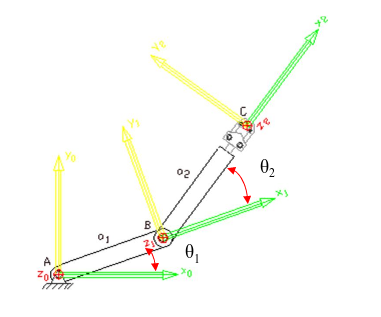
\includegraphics[width=0.9\linewidth]{../../figures/planar_manipulator_DH}
                    %\\[1em]%
                    \caption{manipulator RR} 
                \end{center}                                         
            \end{figure}
        \end{column}%
        
        \hfill%
        
        \begin{column}{.48\textwidth}
            \begin{table}[htb!]
            \centering
            \begin{tabular}{|c|c|c|c|c|}
            \hline 
            i & $a_{i}$ & $\alpha_{i}$ & $d_{i}$ & $\theta_{i}$\tabularnewline[0.3em]
            \hline 
            \hline 
            1 & $a_1$ & $0$ & $0$ & $\theta_{1}$\tabularnewline[0.3em]
            \hline 
            2 & $a_2$ & $0$ & $0$ & $\theta_{2}$\tabularnewline[0.3em]
            \hline 
            \end{tabular}
            \caption{Parametry DH.}
            \label{tab:par_przek}
            \end{table}
            
            Dla prostego modelu mo�emy napisa� od razu r�wnanie po�o�enia ko�c�wki:
            \begin{equation}
                \begin{cases}
                    d_x =a_1 \cdot \cos \theta_1  a_2 \cdot \cos ( \theta_1   \theta_2 ) \\
                    d_y =a_1 \cdot \sin \theta_1  a_2 \cdot \sin ( \theta_1   \theta_2 )
                \end{cases}
            \end{equation}
        \end{column}%
    \end{columns}
}
%
\frame{
    \frametitle{Zadanie proste kinematyki - notacja DH}
    Korzystaj�c z notacji DH:
    \begin{equation}
        T _ { 0 } ^ { 1 } = \left[ \begin{array} { c c c c } { \cos \theta _ { 1 } } & { - \sin \theta _ { 1 } } & { 0 } & { a _ { 1 } \cdot \cos \theta _ { 1 } } \\ { \sin \theta _ { 1 } } & { \cos \theta _ { 1 } } & { 0 } & { a _ { 1 } \cdot \sin \theta _ { 1 } } \\ { 0 } & { 0 } & { 1 } & { 0 } \\ { 0 } & { 0 } & { 0 } & { 1 } \end{array} \right]
    \end{equation}
    \begin{equation}
        T _ { 1 } ^ { 2 } = \left[ \begin{array} { c c c c } { \cos \theta _ { 2 } } & { - \sin \theta _ { 2 } } & { 0 } & { a _ { 2 } \cdot \cos \theta _ { 2 } } \\ { \sin \theta _ { 2 } } & { \cos \theta _ { 2 } } & { 0 } & { a _ { 2 } \cdot \sin \theta _ { 2 } } \\ { 0 } & { 0 } & { 1 } & { 0 } \\ { 0 } & { 0 } & { 0 } & { 1 } \end{array} \right]
    \end{equation}
    czyli
    {\small
    \begin{equation}
        T _ { 0 } ^ { 2 } = T _ { 0 } ^ { 1 } \cdot T _ { 1 } ^ { 2 } = 
        \left[ \begin{array} { c c c c } 
            { \cos (\theta_1 + \theta_2) } & { -\sin (\theta_1 + \theta_2) } & { 0 } & { a_1 \cdot \cos \theta_1 + a_2 \cdot \cos (\theta_1 + \theta_2) } \\ 
            { \sin (\theta_1 + \theta_2) } & { \cos (\theta_1 + \theta_2) } & { 0 } & { a_1 \cdot \sin \theta_1 + a_2 \cdot \sin (\theta_1 + \theta_2) } \\ 
            { 0 } & { 0 } & { 1 } & { 0 } \\ 
            { 0 } & { 0 } & { 0 } & { 1 } 
        \end{array} \right]
    \end{equation}
    }
}
%
\frame{
    \frametitle{Zadanie odwrotne kinematyki - podej�cie geometryczne}
    \begin{columns}[T] % align columns
        \begin{column}{.4\textwidth}
            \begin{figure}[htb!]
                \begin{center}
                    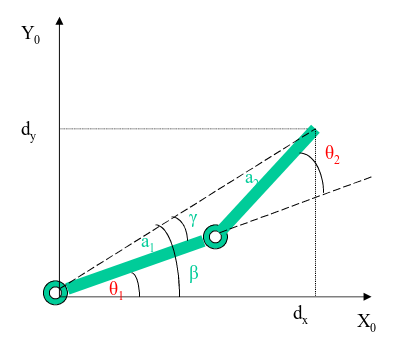
\includegraphics[width=1.0\linewidth]{../../figures/planar_manipulator_inverse_kinematics_ageometric}
                    %\\[1em]%
                    \caption{kinematyka odwrotna geometrycznie} 
                \end{center}                                         
            \end{figure}
        \end{column}%
        
        \hfill%
        
        \begin{column}{.6\textwidth}
            Najpierw wyznaczamy k�t $\theta_2$:
            \begin{equation}
                \begin{split}
                    d _ { x } ^ { 2 } + d _ { y } ^ { 2 } = a _ { 1 } ^ { 2 } + a _ { 2 } ^ { 2 } - 2 \cdot a _ { 1 } \cdot a _ { 2 } \cdot \cos ( \pi - \theta _ { 2 } ) \\
                    d _ { x } ^ { 2 } + d _ { y } ^ { 2 } = a _ { 1 } ^ { 2 } + a _ { 2 } ^ { 2 } + 2 \cdot a _ { 1 } \cdot a _ { 2 } \cdot \cos \theta _ { 2 } \\
                    \cos \theta _ { 2 } = \frac { d _ { x } ^ { 2 } + d _ { y } ^ { 2 } - a _ { 1 } ^ { 2 } - a _ { 2 } ^ { 2 } } { 2 \cdot a _ { 1 } \cdot a _ { 2 } } = L \\
                    \sin \theta _ { 2 } = \pm \sqrt { 1 - L ^ { 2 } } \\
                    \theta _ { 2 } = \operatorname { arctg } \frac { \pm \sqrt { 1 - L ^ { 2 } } } { L }
                \end{split}
            \end{equation}
            Dalej wyznaczamy k�t $\theta_1$:
            \begin{equation}
                \begin{split}
                    \theta _ { 1 } = \beta - \gamma \\
                    \theta _ { 1 } = \operatorname { arctg } \frac { d _ { y } } { d _ { x } } - \operatorname { arctg } \frac { a _ { 2 } \cdot \sin \theta _ { 2 } } { a _ { 1 } + a _ { 2 } \cdot \cos \theta _ { 2 } }
                \end{split}
            \end{equation}
        \end{column}%
    \end{columns}
}
%
\frame{
    \frametitle{Zadanie proste kinematyki pr�dko�ci}
    \begin{equation}
        \begin{cases}
            d _ { x } = a _ { 1 } \cdot \cos \theta _ { 1 } + a _ { 2 } \cdot \cos ( \theta _ { 1 } + \theta _ { 2 } ) \\
            d _ { y } = a _ { 1 } \cdot \sin \theta _ { 1 } + a _ { 2 } \cdot \sin ( \theta _ { 1 } + \theta _ { 2 } )
        \end{cases}
    \end{equation}
    \begin{equation}
        \begin{cases}
            \dot { d } _ { x } = v _ { x } = - a _ { 1 } \cdot \sin \theta _ { 1 } \cdot \dot { \theta } _ { 1 } - a _ { 2 } \cdot \sin ( \theta _ { 1 } + \theta _ { 2 } )\dot( \dot { \theta } _ { 1 } + \dot { \theta } _ { 2 } ) \\
            \dot { d } _ { y } = v _ { y } = a _ { 1 } \cdot \cos \theta _ { 1 } \cdot \hat { \theta _ { 1 } } + a _ { 2 } \cdot \cos ( \theta _ { 1 } + \theta _ { 2 } )\dot( \dot { \theta } _ { 1 } + \dot { \theta } _ { 2 } )
        \end{cases}
    \end{equation}
    {\small
    \begin{equation}
        \left[ \begin{array} { c } 
            { \dot { d } _ { x } } \\ 
            { \dot { d } _ { y } } 
        \end{array} \right] 
        = 
        \left[ \begin{array} { c } 
            { v _ { x } } \\ 
            { v _ { y } } 
        \end{array} \right] 
        =
        \left[ \begin{array} { c c } 
            { - a _ { 1 } \cdot \sin \theta _ { 1 } - a _ { 2 } \cdot \sin ( \theta _ { 1 } + \theta _ { 2 } ) } & { - a _ { 2 } \cdot \sin ( \theta _ { 1 } + \theta _ { 2 } ) } \\ 
            { a _ { 1 } \cdot \cos \theta _ { 1 } + a _ { 2 } \cdot \cos ( \theta _ { 1 } + \theta _ { 2 } ) } & { a _ { 2 } \cdot \cos ( \theta _ { 1 } + \theta _ { 2 } ) } 
        \end{array} \right] 
        \cdot 
        \left[ \begin{array} { c } 
            { \dot { \theta } _ { 1 } } \\ 
            { \dot { \theta } _ { 2 } } 
        \end{array} \right]
    \end{equation}
    }
    Mo�na zauwa�y�, �e:
    \begin{equation}
        J_D
        =
        \left[ \begin{array} { c c } 
            { - a _ { 1 } \cdot \sin \theta _ { 1 } - a _ { 2 } \cdot \sin ( \theta _ { 1 } + \theta _ { 2 } ) } & { - a _ { 2 } \cdot \sin ( \theta _ { 1 } + \theta _ { 2 } ) } \\ 
            { a _ { 1 } \cdot \cos \theta _ { 1 } + a _ { 2 } \cdot \cos ( \theta _ { 1 } + \theta _ { 2 } ) } & { a _ { 2 } \cdot \cos ( \theta _ { 1 } + \theta _ { 2 } ) } 
        \end{array} \right]
    \end{equation}
    wtedy
    \begin{equation}
        \left[ \begin{array} { c } 
            { \dot { d } _ { x } } \\ 
            { \dot { d } _ { y } } 
        \end{array} \right] 
        = 
        \left[ \begin{array} { c } 
            { v _ { x } } \\ 
            { v _ { y } } 
        \end{array} \right] 
        =
        J_D
        \cdot 
        \left[ \begin{array} { c } 
            { \dot { \theta } _ { 1 } } \\ 
            { \dot { \theta } _ { 2 } } 
        \end{array} \right]
    \end{equation}
}
%
\frame{
    \frametitle{Zadanie odwrotne kinematyki pr�dko�ci}
}
%
\frame{
    \frametitle{Model dynamiki}
}
%
\section{Acrobot}
%
\frame{
    \frametitle{Model kinematyki}
    \begin{columns}[T] % align columns
        \begin{column}{.48\textwidth}
            \begin{figure}[htb!]
                \begin{center}
                    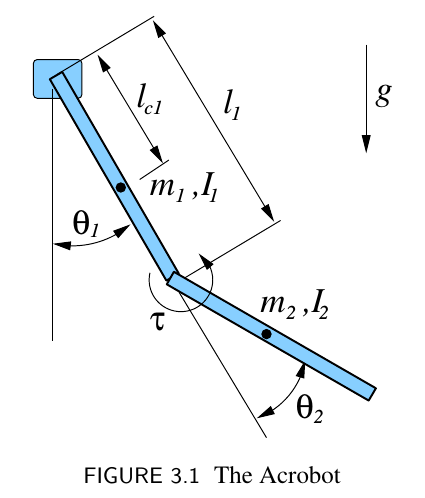
\includegraphics[width=0.9\linewidth]{../../figures/acrobot}
                    %\\[1em]%
                    \caption{acrobot} \label{fig:acrobot}
                \end{center}                                         
            \end{figure}
        \end{column}%
        
        \hfill%
        
        \begin{column}{.48\textwidth}
            Przyjmujemy:\\
            $\theta_1, \theta_2$ - wsp�rz�dne maszynowe.\\
            $q = [\theta_1,\theta_2]^T, x=[q,\dot{q}]^T$
        \end{column}%
    \end{columns}
}
%
\frame{
    \frametitle{Zadanie proste kinematyki}
    
    \begin{equation}
        x_1 =
        \begin{bmatrix}
            l_1 s_1 \\
            -l_1 c_1 \\
        \end{bmatrix}
        , x_2 = x_1 + 
        \begin{bmatrix}
            l_2 s_{12} \\
            -l_2 c_{12} \\
        \end{bmatrix}
        .
    \end{equation}
}
%
\frame{
    \frametitle{Zadanie odwrotne kinematyki}
}
%
\frame{
    \frametitle{Zadanie proste kinematyki pr�dko�ci}
}
%
\frame{
    \frametitle{Zadanie odwrotne kinematyki pr�dko�ci}
}
%
\frame{
    \frametitle{Model dynamiki (1)}
    The energy2 is given by: 
    \begin{align}
        T = T_1 + T_2 \\
        T_1 = \frac{1}{2}I_1\dot{q_1}^2 \\
        T_2 = \frac{1}{2}(m_2 l_1^2 + I_2 + 2 m_2 l_1 l_{c2} c_2)\dot{q_1}^2 + \frac{1}{2}I_2\dot{q_2}^2 + (I_2 + m_2 l_1 l_{c2} c_2)\dot{q_1}\dot{q_2}\\
        U = -m_1 g l_{c1} c_1 - m_2 g (l_1 c_1 + l_2 c_{12})
    \end{align}
    
    Entering these quantities into the Lagrangian yields the equations of motion:
    \begin{align}
        \nonumber
        (I_1 + I_2 + m_2 l_1^2 + 2 m_2 l_1 l_{c2} c_2) \ddot{q_1} + (I_2 + m_2 l_1 l_{c2} c_2) \ddot{q_2} - 2 m_2 l_1 l_{c2} s_2 \dot{q_1} \dot{q_2} \\
        - m_2 l_1 l_{c2} s_2 \dot{q_2}^2 + (m_1 l_{c1} + m_2 l_1) g s_1 + m_2 g l_2 s_{12} = 0 \\
        (I_2 + m_2 l_1 l_{c2} c_2)\ddot{q_1} + I_2 \ddot{q_2} + m_2 l_1 l_{c2} s_2 \dot{q_1}^2 + m_2 g l_2 s_{12} = \tau
    \end{align}
}
%
\frame{
    \frametitle{Model dynamiki(2)}
    
    In standard, manipulator equation form, we have:

    \begin{align}
        H(q) = 
        \begin{bmatrix}
            I_1 + I_2 + m_2 l_1^2 + 2 m_2 l_1 l_{c2} c_2    &   I_2 + m_2 l_1 l_{c2} c_2 \\
            I_2 + m_2 l_1 l_{c2} c_2                        &   I_2 \\
        \end{bmatrix} \\
        C(q, \dot{q}) = 
        \begin{bmatrix}
            - 2 m_2 l_1 l_{c2} s_2 \dot{q_2}                &   - m_2 l_1 l_{c2} s_2 \dot{q_2} \\
            m_2 l_1 l_{c2} s_2 \dot{q_1}                    &   0 \\
        \end{bmatrix} \\
        G(q) = 
        \begin{bmatrix}
            (m_1 l_{c1} + m_2 l_1) g s_1 + m_2 g l_2 s_{12} \\
            m_2 g l_2 s_{12} \\
        \end{bmatrix} \\
        B = 
        \begin{bmatrix}
            0 \\
            1 \\
        \end{bmatrix}
    \end{align}
}
%
\section{Wahad�o odwr�cone}
%
\frame{
    \frametitle{Model kinematyki}
}
%
\frame{
    \frametitle{Zadanie proste kinematyki}
}
%
\frame{
    \frametitle{Zadanie odwrotne kinematyki}
}
%
\frame{
    \frametitle{Zadanie proste kinematyki pr�dko�ci}
}
%
\frame{
    \frametitle{Zadanie odwrotne kinematyki pr�dko�ci}
}
%
\frame{
    \frametitle{Model dynamiki}
}
%

\end{document}
